\def\texpath{tex/}
\def\imgpath{images/}
% !TEX option = --shell-escape

\documentclass[a4paper, 10pt, pdftex, twoside=false, numbers=noenddot, fleqn]{scrbook}

	\input{\texpath header}

	\graphicspath{{\imgpath}}
	\addbibresource{bib/articles.bib}

	
\begin{document}

	\input{\texpath titlepage}
	\chapter*{Vorwort}
\addcontentsline{toc}{chapter}{Vorwort} % Fügt das Vorwort ins Inhaltsverzeichnis ein

Die vorliegende Bachelorarbeit entstand im Rahmen meines Studiums der Informatik (B.Sc.) an der Hochschule Bochum. Das Thema „Analyse und Entwicklung eines Systems zur Visualisierung von Mitarbeitendengesprächsdaten“ wurde gewählt, da es sowohl ein spannendes und praxisnahes Forschungsfeld darstellt als auch direkt mit einer von mir entwickelten Anwendung verbunden ist. Diese Anwendung entstand ursprünglich aus einem konkreten Bedarf in der Praxis und wurde im Laufe der Arbeit kontinuierlich weiterentwickelt und verfeinert, um den wissenschaftlichen und praktischen Anforderungen gerecht zu werden.

Die Entwicklung dieses Systems bot nicht nur einen tiefen Einblick in moderne Technologien und deren Anwendung im HR-Bereich, sondern auch die Möglichkeit, praxisnahe Lösungen für komplexe Probleme zu erarbeiten. Besonders die Verbindung von theoretischem Wissen mit praktischen Umsetzungen stellte einen zentralen Lerngewinn dar.

Die Arbeit unterstreicht die Bedeutung einer interdisziplinären Herangehensweise, bei der technologische Innovationen auf die Bedürfnisse der Arbeitswelt abgestimmt werden. Moderne HR-Management-Systeme können nicht nur die Effizienz von Prozessen steigern, sondern auch die Qualität von Entscheidungen verbessern und eine transparente Kommunikation zwischen Führungskräften und Mitarbeitenden fördern. 

Abschließend verdeutlicht diese Arbeit, wie moderne Technologien und datenbasierte Visualisierungen die Praxis von Mitarbeitendengesprächen nachhaltig transformieren können. Die gewonnenen Einsichten und praktischen Erfahrungen bieten eine solide Grundlage, um diese Konzepte in zukünftigen Projekten und beruflichen Aufgabenfeldern weiterzuentwickeln. Damit leistet die Arbeit einen relevanten Beitrag zur Weiterentwicklung moderner HR-Strategien und bietet zugleich eine fundierte Basis für zukünftige Forschung und Praxis.

Mein besonderer Dank gilt meiner Erstprüferin, Frau Anja Tenberge, für ihre konstruktive Unterstützung und hilfreichen Anregungen. Ebenso danke ich Herrn Sascha Bajonczak als Zweitprüfer sowie allen Kolleginnen und Kollegen, die mich während der Erstellung dieser Arbeit unterstützt haben. Nicht zuletzt möchte ich meiner Familie und meinen Freunden danken, die mir durch ihre Unterstützung in dieser intensiven Zeit stets den Rücken gestärkt haben.

\vspace{1cm}

\begin{flushright}
Düsseldorf, Januar 2025 \\
Berk-Can Atesoglu
\end{flushright}

	\tableofcontents

    \listoffigures
    \newpage

    \listoftables
    \newpage

      \section*{Abkürzungsverzeichnis}
\label{abkuerzungen}
\begin{tabbing}
MAG \hspace{1cm} \= Mitarbeitergespräch \\
API \> Application Programming Interface \\
JSON \> JavaScript Object Notation \\
HR \> Human Resources \\
CI/CD \> Continuous Integration / Continuous Deployment \\
JWT \> JSON Web Token \\
MSAL \> Microsoft Authentication Library \\
AAD \> Azure Active Directory \\
SQL \> Structured Query Language \\
OData \> Open Data Protocol \\
DTO \> Data Transfer Object \\
EF Core \> Entity Framework Core \\
REST \> Representational State Transfer \\
UI \> User Interface \\
DOM \> Document Object Model \\
MFA \> Multi-Factor Authentication \\
HMR \> Hot Module Replacement \\
ER \> Entity Relationship \\
XSS \> Cross-Site Scripting \\
CRUD \> Create, Read, Update, Delete \\
HTTP \> Hypertext Transfer Protocol \\
SQL \> Structured Query Language \\
PROD\> Production \\
ADD  \> Azure Active Directory \\
IDE \> integrierte Entwicklungsumgebung \\
\end{tabbing}


	\chapter{Einleitung} \label{chap:einleitung}

Die Qualität und Effizienz von Mitarbeitendengesprächen sind essenziell für den Erfolg eines Unternehmens. Solche Gespräche schaffen eine Plattform für Feedback, Leistungsbewertungen, die gemeinsame Festlegung von Zielen und die Planung individueller Entwicklungsmöglichkeiten. Regelmäßige  Gespräche tragen nicht nur zur Stärkung der Mitarbeitendenbindung bei, sondern fördern auch die Produktivität und die strategische Ausrichtung des Unternehmens, indem sie die Ziele der Organisation mit den Bedürfnissen der Mitarbeitenden in Einklang bringen \cite{Schober2008, Bryson2011}.

In einer zunehmend datengetriebenen Welt wird es immer wichtiger, große Datenmengen nicht nur zu sammeln, sondern auch sinnvoll zu nutzen. Gerade im Bereich Human Resources (\hyperref[abkuerzungen]{HR}) bleiben die Ergebnisse von Mitarbeitendengesprächen oft ungenutzt, da sie in unstrukturierter Form vorliegen. Dadurch entgehen Unternehmen wertvolle Einblicke, die zur Förderung der Mitarbeitendenentwicklung und zur Optimierung von HR-Strategien beitragen könnten \cite{Kirk2016}. Der Einsatz moderner Visualisierungstools bietet hier eine Lösung, indem er die Darstellung und Analyse solcher Daten erleichtert und datenbasierte Entscheidungen unterstützt.

Trotz der zunehmenden Digitalisierung in Unternehmen existiert eine Forschungslücke in der Verbindung zwischen datengetriebener Analyse und der praktischen Umsetzung in Mitarbeitendengesprächen. Während Studien die Vorteile datenbasierter Ansätze im (\hyperref[abkuerzungen]{HR})-Management betonen \cite{Evergreen2016}, fehlen praxisnahe Beispiele, die moderne Technologien wie interaktive Visualisierungen und cloudbasierte Datenverarbeitung zur Optimierung solcher Gespräche nutzen. Diese Arbeit schließt diese Lücke, indem sie ein System entwickelt, das datengetriebene Erkenntnisse für Mitarbeitendengespräche praktisch anwendbar macht.

Die Inhalte der Arbeit wurden in Zusammenarbeit mit der Realcore Services GmbH entwickelt, einem führenden IT-Dienstleister, der sich auf innovative Lösungen für die Optimierung interner Prozesse spezialisiert hat. Ziel der Arbeit ist es, ein modernes und benutzerfreundliches Reporting-Tool zu entwickeln, das speziell für die Analyse und Visualisierung von Daten aus Mitarbeitendengesprächen konzipiert ist. Dabei werden technologische Ansätze wie React, .NET Core und Microsoft Azure eingesetzt, um eine flexible, skalierbare und sichere Plattform zu schaffen.

Die zentrale Forschungsfrage dieser Arbeit lautet: \begin{quote} Wie können datenbasierte Visualisierungen und moderne Technologien zur Optimierung von Mitarbeitendengesprächen beitragen und deren Effizienz sowie strategische Relevanz für Unternehmen erhöhen? \end{quote}

Wissenschaftlich leistet diese Arbeit einen Beitrag zur Integration von datengetriebenen Visualisierungen und modernen Technologien in den Kontext von Mitarbeitendengesprächen. Sie untersucht nicht nur die technische Machbarkeit solcher Systeme, sondern auch die Akzeptanz und Praxistauglichkeit in der realen Arbeitswelt. Dadurch liefert sie wertvolle Erkenntnisse für zukünftige Forschung und Entwicklung in diesem Bereich.

Die zentralen Herausforderungen liegen dabei in der effizienten Verarbeitung von Daten aus Mitarbeitendengesprächen, die oft in fragmentierter oder unstrukturierter Form vorliegen. Ziel ist es, diese Daten zu organisieren und durch interaktive Visualisierungen wie Donut-Diagramme und Radarcharts zugänglich zu machen, um Führungskräfte und (\hyperref[abkuerzungen]{HR})-Abteilungen bei der Entscheidungsfindung zu unterstützen \cite{Evergreen2016}. Neben der technischen Umsetzung wird auch untersucht, wie das entwickelte System durch benutzerzentrierte Gestaltung Akzeptanz und Praxistauglichkeit erhöhen kann.

Die vorliegende Arbeit gliedert sich wie folgt: Im Kapitel~\ref{chap:theoretische-grundlagen} werden die theoretischen Grundlagen vorgestellt, die die Bedeutung von Mitarbeitendengesprächen, die Rolle der Datenvisualisierung und die eingesetzten Technologien umfassen. Kapitel~\ref{chap:analysephase} widmet sich der Analyse der Anforderungen durch Stakeholder-Interviews und einen Vergleich bestehender Lösungen. Die Konzeption des Systems, einschließlich der Systemarchitektur, des Datenmodells und der Sicherheitsmaßnahmen, wird im Kapitel~\ref{chap:konzeption} beschrieben. Kapitel~\ref{chap:implementierung} behandelt die technische Implementierung, wobei auf Herausforderungen und deren Lösungen eingegangen wird. Im Kapitel~\ref{chap:evaluation} wird das System evaluiert, indem Funktionstests und Usability-Analysen durchgeführt werden. Abschließend fasst Kapitel~\ref{chap:fazit} die Ergebnisse zusammen und gibt einen Ausblick auf mögliche Weiterentwicklungen.

Diese Arbeit soll insgesamt nicht nur zur Effizienzsteigerung von Mitarbeitendengesprächen beitragen, sondern auch zeigen, wie datenbasierte Ansätze die strategische Ausrichtung und Entscheidungsfindung in Unternehmen nachhaltig unterstützen können. Darüber hinaus liefert sie praktische Erkenntnisse, wie innovative Technologien die Digitalisierung von (\hyperref[abkuerzungen]{HR})-Prozessen vorantreiben können.
	\chapter{Theoretische Grundlagen}
\label{chap:theoretische-grundlagen}

Die individuelle Entwicklung von Mitarbeitenden erfolgt maßgeblich durch zielgerichtete Gespräche und datengestützte Feedbackprozesse. Die folgenden Abschnitte beleuchten die Bedeutung von Mitarbeitendengesprächen, die Rolle der Datenvisualisierung in diesem Kontext sowie die technologische Basis für deren Implementierung. Hierbei wird auf die Verknüpfung von strategischen Unternehmenszielen und persönlichen Entwicklungsmöglichkeiten eingegangen, um eine nachhaltige Verbesserung der Teamdynamik und Leistungseffizienz zu fördern. Diese theoretischen Grundlagen bilden das Fundament für die anschließende Analyse und Entwicklung eines optimalen Systems zur Visualisierung von Mitarbeitendengesprächsdaten.

\section{Mitarbeitendengespräche und ihre Bedeutung}
Mitarbeitendengespräche, auch als „MAG“ bezeichnet, umfassen alle Gespräche, die Vorgesetzte mit Mitarbeitenden zu spezifischen Anlässen führen. Diese Gespräche dienen dazu:
\begin{itemize}
    \item Informationen auszutauschen,
    \item Wertschätzung, Lob oder Kritik zu äußern und
    \item Entwicklungsziele zu formulieren \cite{schober2008}.
\end{itemize}

Ein strukturierter Ablauf solcher Gespräche fördert die innerbetriebliche Kommunikation und die Bindung der Mitarbeitenden an das Unternehmen. Typische Elemente von Mitarbeitendengesprächen sind:
\begin{itemize}
    \item \textbf{Bewertung der bisherigen Zielerreichung:} Analyse des Fortschritts in Bezug auf zuvor gesetzte Ziele \cite{duarte2012performance}.
    \item \textbf{Setzen neuer Ziele:} Definition von SMART-Zielen (spezifisch, messbar, akzeptiert, realistisch, terminiert), die eine klare Richtung für die zukünftige Arbeit vorgeben \cite{duarte2012performance}.
    \item \textbf{Diskussion von Entwicklungsmaßnahmen:} Identifikation von Schulungsbedarf und Weiterbildungsangeboten zur Förderung von persönlichem und beruflichem Wachstum \cite{bryson2011employee}.
\end{itemize}

Eine strukturierte Gesprächsführung kann Verzerrungen durch subjektive Einschätzungen minimieren, insbesondere durch den Einsatz datenbasierter Methoden \cite{heikkila2018}. Dies unterstützt Führungskräfte dabei, fundierte Entscheidungen zu treffen, die sowohl die individuellen Ziele der Mitarbeitenden als auch die strategischen Unternehmensziele berücksichtigen \cite{barton2012}.

\section{Relevanz von Datenvisualisierung}
Datenvisualisierung ist ein zentraler Bestandteil moderner Analytik und spielt eine entscheidende Rolle bei der Interpretation komplexer Informationen. Sie unterstützt Führungskräfte dabei, datenbasierte Entscheidungen zu treffen, indem sie große Datenmengen in verständliche visuelle Darstellungen umwandelt \cite{kirk2016data}. 

\subsection*{Hauptvorteile der Datenvisualisierung}
\begin{itemize}
    \item \textbf{Verbesserte Entscheidungsfindung:} Daten werden schneller und effizienter interpretiert \cite{kirk2016data}.
    \item \textbf{Erkennung von Trends und Abweichungen:} Historische und aktuelle Daten können leicht verglichen werden, um Entwicklungen zu identifizieren \cite{ware2012information}.
    \item \textbf{Kommunikation und Präsentation:} Visualisierte Daten fördern eine klare Kommunikation zwischen Teams und Stakeholdern \cite{evergreen2016effective}.
\end{itemize}

Im Kontext von Mitarbeitendengesprächen sind Radarcharts und Donutcharts besonders geeignet:
\begin{itemize}
    \item \textbf{Radarcharts:} Vergleich mehrerer Leistungsdimensionen wie Teamarbeit, Effizienz und Pünktlichkeit \cite{heikkila2018}.
    \item \textbf{Donutcharts:} Übersicht über den Status von Zielvereinbarungen oder Fortschritten \cite{evergreen2016effective}.
\end{itemize}
\newpage

\section{Technologische Basis}
Die technologische Basis für ein System zur Visualisierung von Mitarbeitendengesprächsdaten ist entscheidend für dessen Funktionalität, Benutzerfreundlichkeit und Skalierbarkeit. Die ausgewählten Technologien umfassen:

\begin{itemize}
    \item \textbf{React:} Eine JavaScript-Bibliothek für die komponentenbasierte Entwicklung dynamischer Benutzeroberflächen \cite{stefanov2021react}.
    \item \textbf{TypeScript:} Erweiterung von JavaScript mit statischer Typisierung zur Verbesserung der Codequalität \cite{typeScriptDocumentation}.
    \item \textbf{.NET Core:} Plattformübergreifendes Framework für die Entwicklung skalierbarer und leistungsstarker Backend-Anwendungen \cite{microsoftDotNet}.
    \item \textbf{MSSQL:} Eine cloudbasierte Datenbanklösung, die Sicherheit und Skalierbarkeit für große Datenmengen bietet \cite{azureDocumentation}.
    \item \textbf{Azure Ressourcen:} Verschiedene Dienste von Microsoft Azure wurden in der Implementierung genutzt, um eine umfassende und skalierbare Lösung zu gewährleisten:
    \begin{itemize}
       \item \textbf{Entra ID (ehemals Azure Active Directory):} Entra ID bietet umfassende Authentifizierungs- und Autorisierungsdienste, einschließlich Multi-Faktor-Authentifizierung und rollenbasierter Zugriffskontrolle. Studien zeigen, dass die Verwendung solcher Systeme die Sicherheit und Effizienz in Unternehmen erheblich erhöht \cite{microsoftEntraID, woods2020authentication}.
\item \textbf{Microsoft Graph API:} Diese API ermöglicht die Interaktion mit verschiedenen Microsoft-Diensten, wie Benutzerdatenabfragen und Kalenderintegration. Laut aktuellen Forschungsergebnissen ist die Nutzung von Graph APIs ein Schlüssel für die Automatisierung und Integration in moderne Softwarelandschaften \cite{microsoftGraphAPI, smith2021graph}.
\item \textbf{Application Insights:} Ein Telemetriedienst, der zur Überwachung und Analyse der Anwendungsleistung eingesetzt wird. Studien belegen, dass Application Insights eine signifikante Verbesserung in der Fehlerdiagnose und Performanceanalyse moderner Cloud-Anwendungen ermöglicht \cite{microsoftAppInsights, li2021monitoring}.
\item \textbf{App Services:} Ein Telemetriedienst, der zur Überwachung und Analyse der Anwendungsleistung eingesetzt wird. Studien belegen, dass Application Insights eine signifikante Verbesserung in der Fehlerdiagnose und Performanceanalyse moderner Cloud-Anwendungen ermöglicht 
\item \textbf{Container Registry:} Ein Telemetriedienst, der zur Überwachung und Analyse der Anwendungsleistung eingesetzt wird. Studien belegen, dass Application Insights eine signifikante Verbesserung in der Fehlerdiagnose und Performanceanalyse moderner Cloud-Anwendungen ermöglicht 

\end{itemize}

\item \textbf{Git:} Verschiedene Dienste von Microsoft Azure wurden in der Implementierung genutzt, um eine umfassende und skalierbare Lösung zu gewährleisten
\item \textbf{DevOps:} Verschiedene Dienste von Microsoft Azure wurden in der Implementierung genutzt, um eine umfassende und skalierbare Lösung zu gewährleisten:
    \begin{itemize}    
    \item \textbf{CI/CD-Pipeline:} Mit Azure DevOps werden automatisierte Continuous Integration und Continuous Deployment (CI/CD) umgesetzt, um Entwicklungs- und Bereitstellungsprozesse zu optimieren. Aktuelle Veröffentlichungen zeigen, dass CI/CD-Pipelines die Bereitstellungszeit um bis zu 50 \% reduzieren können \cite{azureDevOps, fowler2020continuous}.
     \item \textbf{HBS-Masstransit Artefakt:} Mit Azure DevOps werden automatisierte Continuous Integration und Continuous Deployment (CI/CD) umgesetzt, um Entwicklungs- und Bereitstellungsprozesse zu optimieren. Aktuelle Veröffentlichungen zeigen, dass CI/CD-Pipelines die Bereitstellungszeit um bis zu 50 \% reduzieren können \cite{azureDevOps, fowler2020continuous}.

      \item \textbf{Repository:} Mit Azure DevOps werden automatisierte Continuous Integration und Continuous Deployment (CI/CD) umgesetzt, um Entwicklungs- und Bereitstellungsprozesse zu optimieren. Aktuelle Veröffentlichungen zeigen, dass CI/CD-Pipelines die Bereitstellungszeit um bis zu 50 \% reduzieren können \cite{azureDevOps, fowler2020continuous}.
\end{itemize}


\subsection*{Integration der Technologien}
Die Kombination aus React und TypeScript ermöglicht die Entwicklung einer flexiblen und responsiven Benutzeroberfläche. Backend-seitig sorgt .NET Core für eine skalierbare und performante Architektur, während MS SQL als sichere Speicherlösung dient. Die enge Verzahnung dieser Technologien gewährleistet eine effiziente Datenverarbeitung und nahtlose Integration in bestehende Infrastrukturen \cite{microsoftAzure}.

\section{Zusammenfassung}
Mitarbeitendengespräche, unterstützt durch Datenvisualisierung und moderne Technologien, bieten erhebliches Potenzial zur Förderung der Teamdynamik und zur Erreichung von Unternehmenszielen. Die theoretischen Grundlagen zeigen, dass die Kombination von strukturierten Gesprächen, datenbasierter Entscheidungsfindung und technologischen Innovationen die Basis für ein effizientes und skalierbares System bildet.


	\chapter{Analysephase}
\label{chap:analysephase}

\section{Anforderungen} Die Anforderungen an das geplante Tool wurden auf Basis von Stakeholder-Interviews und einer Analyse bestehender Lösungen definiert. Ziel war es, eine effektive, skalierbare und benutzerfreundliche Lösung zu entwerfen, die den spezifischen Anforderungen von Führungskräften und (\hyperref[abkuerzungen]{HR})-Managern entspricht.

Um die Funktionalität und Effizienz des Systems sicherzustellen, wurden sowohl funktionale als auch nicht-funktionale Anforderungen formuliert. Die funktionalen Anforderungen umfassen Kernfunktionen wie interaktive Visualisierungen, Datenmanagement und Benutzerverwaltung, während nicht-funktionale Anforderungen Aspekte wie Sicherheit, Performance und Skalierbarkeit adressieren.

Das System soll die Visualisierung von Daten durch interaktive Donut- und Radarcharts ermöglichen, um Trends und Leistungskennzahlen übersichtlich darzustellen \cite{kirk2016data}. Gleichzeitig soll ein strukturiertes Datenmanagement den Import, die Speicherung und die Bearbeitung von Gesprächsdaten sicherstellen, um Nachverfolgbarkeit und Konsistenz zu gewährleisten \cite{bryson2011employee}. Zusätzlich wird ein Exportmodul benötigt, um Berichte in Formaten wie Excel und PDF für weiterführende Analysen bereitzustellen. Die Benutzerverwaltung des Tools ermöglicht differenzierte Zugriffskontrollen, die sensible Daten schützen und rollenbasierten Zugriff gewährleisten \cite{duarte2012performance}.

Nicht-funktionale Anforderungen konzentrieren sich auf die Qualität des Tools. Die Performance des Systems muss auch bei großen Datenmengen eine schnelle Verarbeitung gewährleisten. Die Skalierbarkeit soll sicherstellen, dass das System mit wachsender Nutzer- und Datenanzahl effizient arbeitet. Zudem ist die Sicherheit durch moderne Authentifizierungs- und Verschlüsselungsmethoden zu gewährleisten, um sensible Informationen zu schützen \cite{sommerville2015, nygard2018, schneier1996}.


\section{Stakeholder-Interviews und Umfragen}
Zur Ermittlung der Anforderungen wurden zwischen März und Mai 2024 halbstrukturierte Interviews mit 15 Führungskräften und (\hyperref[abkuerzungen]{HR})-Managern aus verschiedenen Abteilungen des Unternehmens durchgeführt. Die Teilnehmenden wurden gezielt ausgewählt, um unterschiedliche Benutzergruppen und ihre Perspektiven abzudecken, darunter Vertreter aus operativen und strategischen Bereichen. Die Gespräche dauerten durchschnittlich 45 Minuten und umfassten Themen wie relevante Daten für Entscheidungsfindungen, Herausforderungen bestehender Tools und essenzielle Funktionen für die tägliche Arbeit \cite{bryman2015social}.

Die Antworten wurden qualitativ analysiert, um zentrale Anforderungen und Prioritäten zu identifizieren \cite{flick2009qualitative}. Die Ergebnisse zeigten, dass Datensicherheit und benutzerfreundliche Visualisierungen höchste Priorität hatten. Darüber hinaus bestand der Wunsch nach einer dynamischen Benutzeroberfläche mit Echtzeit-Updates. Visualisierungen sollten Trends und Muster schnell erkennbar machen, und die Benutzeroberfläche sollte stets aktuelle Daten bereitstellen. Gleichzeitig wurde die Bedeutung strikter Anforderungen an den Schutz sensibler Gesprächsdaten betont \cite{kirk2016data, bryson2011employee}.

\begin{figure}[h!]
\centering
Die Abbildung illustriert die Häufigkeit, mit der 32 Mitarbeitende bestimmte Anforderungen während der Stakeholder-Interviews genannt haben. Dabei zeigt sich, dass Datensicherheit die höchste Priorität hatte, gefolgt von der Nachfrage nach Visualisierungen und Echtzeit-Updates. Diese Ergebnisse verdeutlichen die zentralen Schwerpunkte, die bei der Entwicklung des Tools berücksichtigt werden sollten.

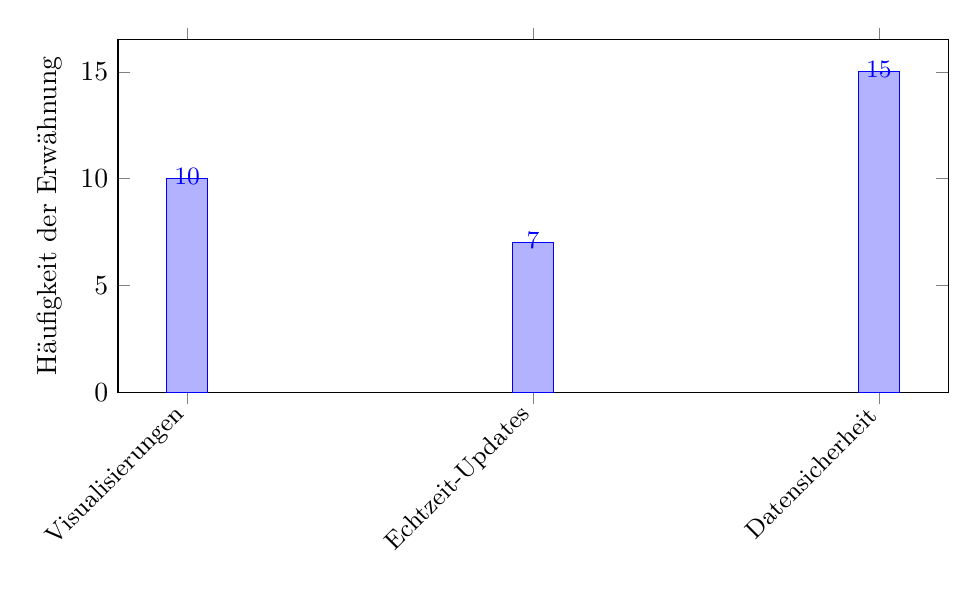
\begin{tikzpicture} \begin{axis}[ width=\textwidth, height=0.5\textwidth, ybar, bar width=15pt, ylabel={Häufigkeit der Erwähnung}, symbolic x coords={Visualisierungen, Echtzeit-Updates, Datensicherheit}, xtick=data, x tick label style={font=\small, rotate=45, anchor=east}, ymin=0, nodes near coords, nodes near coords style={font=\small, anchor=mid}, ] \addplot coordinates {(Visualisierungen,10) (Echtzeit-Updates,7) (Datensicherheit,15)}; \end{axis} \end{tikzpicture} \caption{Häufigkeit genannter Anforderungen aus Stakeholder-Interviews.} \label{fig:stakeholder_results_barchart} \end{figure}

\section{Einordnung bestehender Lösungen}
Zur Bewertung der vorhandenen Marktsituation wurden die Tools HRworks und Evalea analysiert, die als etablierte Lösungen im (\hyperref[abkuerzungen]{HR})-Bereich gelten. Beide Systeme bieten spezifische Funktionen zur Unterstützung von HR-Prozessen, weisen jedoch Einschränkungen in der Visualisierung von Daten und der Anpassungsfähigkeit an unternehmensspezifische Anforderungen auf. HRworks fokussiert auf die allgemeine Verwaltung von (\hyperref[abkuerzungen]{HR})-Daten und bietet Basisfunktionen wie eine intuitive Benutzeroberfläche und 360°-Feedback-Optionen. Evalea hingegen punktet durch umfangreichere Reporting-Funktionen und anpassbare Gesprächsleitfäden. Beide Tools bieten jedoch keine interaktiven Visualisierungsmöglichkeiten, wie sie für das geplante System vorgesehen sind.

Die Analyse in Abbildung~\ref{fig:hrworks_evalea_comparison} zeigt, dass Evalea in den Kategorien Funktionalität \\und Reporting gegenüber HRworks überlegen ist. Allerdings fehlen bei beiden Lösungen Echtzeit-Visualisierungen, die für datenintensive Analysen und strategische Entscheidungen unverzichtbar sind. Die Ergebnisse verdeutlichen, dass \\Echtzeit-Visualisierungen und eine tiefergehende Integration in bestehende Systeme entscheidende Lücken darstellen, die das geplante System adressieren soll.

\begin{figure}[h!]
\centering
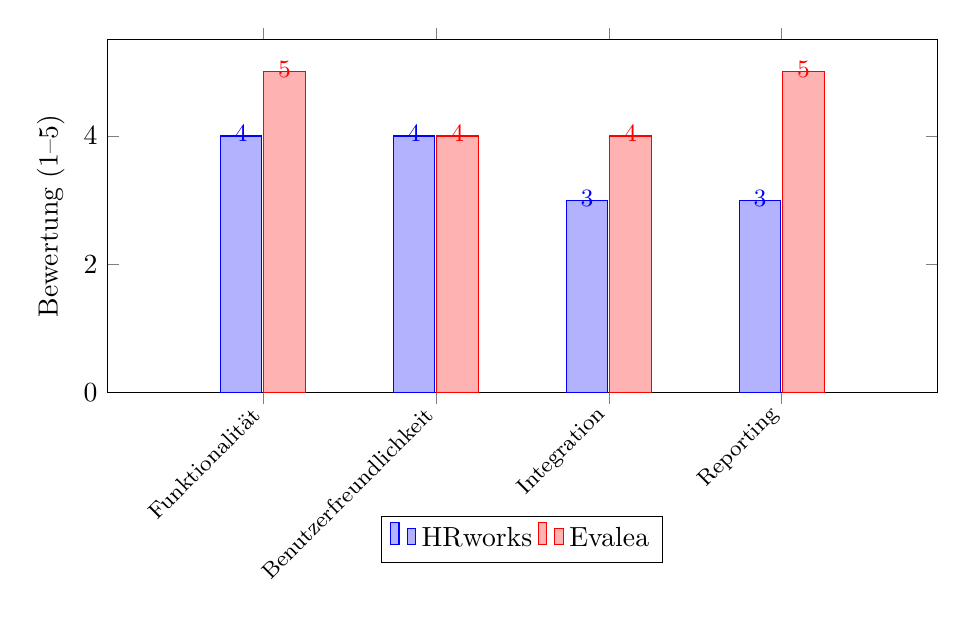
\begin{tikzpicture}
\begin{axis}[ width=\textwidth, height=0.5\textwidth, ybar=0.7pt, bar width=15pt, enlarge x limits=0.3, ylabel={Bewertung (1–5)}, symbolic x coords={Funktionalität, Benutzerfreundlichkeit, Integration, Reporting}, xtick=data, x tick label style={font=\footnotesize, rotate=45, anchor=east}, ymin=0, ymax=5.5, nodes near coords, nodes near coords style={font=\small, anchor=mid}, legend style={at={(0.5,-0.35)}, anchor=north, legend columns=-1}, legend cell align={left} ] \addplot[blue,fill=blue!30] coordinates { (Funktionalität,4) (Benutzerfreundlichkeit,4) (Integration,3) (Reporting,3) }; \addplot[red,fill=red!30] coordinates { (Funktionalität,5) (Benutzerfreundlichkeit,4) (Integration,4) (Reporting,5) }; \legend{HRworks, Evalea} \end{axis} \end{tikzpicture} \caption{Vergleich zwischen HRworks und Evalea in verschiedenen Kategorien.} \label{fig:hrworks_evalea_comparison} \end{figure}

Die Analysephase verdeutlichte, dass das geplante System eine klare Lücke in den bestehenden HR-Tools schließen kann. Die Anforderungen aus den Stakeholder-Interviews sowie die Evaluation bestehender Lösungen bilden die Grundlage für die Entwicklung eines Systems, das durch benutzerfreundliche Visualisierungen, Sicherheit und Skalierbarkeit überzeugt. Dies ermöglicht eine effektive Unterstützung von (\hyperref[abkuerzungen]{HR})-Abteilungen bei datenbasierten Entscheidungen und der strategischen Planung.
	\chapter{Konzeption des Systems}
\label{chap:konzeption}

\section{Systemarchitektur}
\subsection{Architekturüberblick}
\begin{itemize}
    \item \textbf{Frontend:} Benutzerinteraktionen und Visualisierung mit React.
    \item \textbf{Backend:} Datenverarbeitung und -verwaltung mit .NET Core.
    \item \textbf{Datenbank:} Speicherung der Daten in Azure SQL.
    \item \textbf{Datenfluss:} Kommunikation zwischen Frontend und Backend über RESTful APIs.
\end{itemize}

\section{Datenmodell}
\begin{itemize}
    \item \textbf{Mitarbeiterdaten:} ID, Name, Position.
    \item \textbf{Gesprächsdaten:} Mitarbeiter-ID, Datum, Bewertungspunkte.
    \item \textbf{Visualisierungsparameter:} Diagrammtypen, Datenquellen.
\end{itemize}
Beziehungen werden mithilfe eines UML-Diagramms dargestellt.

\section{Visualisierungsdesign}
\subsection{Diagrammtypen}
\begin{itemize}
    \item \textbf{Donut-Charts:} Überblick über den Status von Zielvereinbarungen.
    \item \textbf{Radarcharts:} Vergleich der Leistung in verschiedenen Kategorien.
\end{itemize}

\subsection{UI/UX-Überlegungen}
\begin{itemize}
    \item Klar strukturierte Benutzeroberfläche.
    \item Fokus auf einfache Bedienung und schnelle Navigation.
\end{itemize}

\section{Sicherheitskonzepte}
\begin{itemize}
    \item \textbf{Datenverschlüsselung:} SSL für Datenübertragung, AES-256 für Datenspeicherung.
    \item \textbf{Benutzerrechte:} Zugriffskontrolle basierend auf Rollen (z. B. Admin, Benutzer).
    \item \textbf{Authentifizierung:} OAuth 2.0 für sichere Anmeldung.
\end{itemize}
	\chapter{Implementierung}
\label{chap:implementierung}

\section{Technologische Basis}
Die Implementierung basiert auf einer sorgfältig ausgewählten technologischen Basis, die modernste Tools und Frameworks kombiniert, um eine effiziente und skalierbare Lösung zu gewährleisten. Die wichtigsten Technologien sind:
\begin{itemize}
    \item \textbf{Frontend:} Entwicklung mit React und TypeScript. Material-UI wird für konsistente UI-Komponenten genutzt, während Vite für schnelle Build- und Entwicklungsprozesse sorgt.
    \item \textbf{Backend:} Aufbau von RESTful APIs mit .NET Core. Middleware-Services ermöglichen Authentifizierung, Fehlerbehandlung und Protokollierung.
    \item \textbf{Datenbank:} Relationale Modellierung und Abfragen in Azure SQL mit Entity Framework Core für nahtlosen Datenzugriff.
    \item \textbf{DevOps:} Automatisierte CI/CD-Pipelines mit Azure Pipelines, die den Entwicklungs- und Bereitstellungsprozess optimieren.
\end{itemize}

\section{Detailierte Architektur}
\subsection{Frontend-Architektur}
Das Frontend wurde mit einer komponentenbasierten Architektur entwickelt, die eine modulare und wiederverwendbare Struktur ermöglicht:
\begin{itemize}
    \item \textbf{Komponenten:} Jedes UI-Element wurde als eigenständige Komponente entwickelt, um Wartbarkeit und Wiederverwendbarkeit zu maximieren.
    \item \textbf{State-Management:} Für die Verwaltung globaler Zustände kommen Redux Toolkit und Zustand zum Einsatz.
    \item \textbf{Datenvisualisierung:} ApexCharts und React-AäpexCharts werden zur Darstellung von Donut- und Radarcharts verwendet.
\end{itemize}

\begin{minted}[linenos, frame=single, fontsize=\small, caption=Beispiel einer React-Komponente, label=lst:react_component]{javascript}
import React from 'react';
import { Chart } from 'react-apexcharts';

const RadarChart = () => {
  const data = {
    labels: ['Teamarbeit', 'Effizienz', 'Pünktlichkeit', 'Innovation'],
    datasets: [
      {
        label: 'Mitarbeiter A',
        data: [80, 90, 70, 85],
        backgroundColor: 'rgba(54, 162, 235, 0.2)',
        borderColor: 'rgba(54, 162, 235, 1)',
        borderWidth: 2,
      },
    ],
  };

  return <Chart options={data} type="radar" />;
};

export default RadarChart;
\end{minted}


\section{Backend-Architektur}
Das Backend basiert auf einer mehrschichtigen Architektur, die eine klare Trennung von Verantwortlichkeiten gewährleistet. Diese Architektur stellt die Grundlage für eine effiziente und skalierbare Verarbeitung von Mitarbeitendengesprächsdaten dar.

\subsection{Technologische Basis}
Die Entwicklung des Backends erfordert eine fundierte Auswahl moderner Technologien und Methoden, um zentrale Anforderungen wie Sicherheit, Performanz, Skalierbarkeit und Datenverarbeitung zu erfüllen. Folgende Komponenten sind integraler Bestandteil der Implementierung:
\begin{itemize}
    \item \textbf{API-Entwicklung:} Implementierung von RESTful APIs mit .NET Core, die eine zuverlässige und standardisierte Datenübertragung ermöglichen.
    \item \textbf{Cloud-Technologien:} Integration von Microsoft Azure-Diensten wie Azure SQL und Azure Service Bus zur Unterstützung asynchroner Kommunikation und Datenverarbeitung.
    \item \textbf{Sicherheitsmechanismen:} Einsatz von Azure Active Directory (AAD) für Multi-Faktor-Authentifizierung und rollenbasierte Zugriffskontrolle.
    \item \textbf{Datenverarbeitung:} Nutzung skalierbarer Algorithmen zur Aggregation und Transformation komplexer Datenstrukturen.
\end{itemize}

\subsection{Komponenten der Backend-Architektur}
\begin{itemize}
    \item \textbf{Controller-Schicht:} Zuständig für die Verarbeitung von Anfragen und das Routing.
    \item \textbf{Service-Schicht:} Implementiert die Geschäftslogik und ist für Datenverarbeitung und Validierung verantwortlich.
    \item \textbf{Repository-Schicht:} Ermöglicht den Zugriff auf die Datenbank mithilfe von Entity Framework Core.
    \item \textbf{Middleware:} Authentifizierung und Fehlerbehandlung werden zentral über Middleware-Komponenten gesteuert.
\end{itemize}

\subsection{API-Endpunkte}
Zur Interaktion mit den Daten des Systems wurden verschiedene API-Endpunkte implementiert. Die folgende Tabelle listet die wesentlichen HTTP-Methoden und URLs zur Manipulation von Ressourcen:

\begin{table}[H]
\caption{HTTP-Methoden und URLs zur Manipulation von Ressourcen}
\label{table:http-methods}
\raggedright
{\scriptsize Quelle: Eigene Darstellung} \\[0.3em]
\renewcommand{\arraystretch}{1.1} % Leichter reduzierter Zeilenabstand
\setlength{\tabcolsep}{1.8pt} % Weiter verringerter horizontaler Zellabstand
\begin{tabularx}{\textwidth}{>{\centering\arraybackslash}m{2cm}|>{\centering\arraybackslash}m{5.5cm}|>{\raggedright\arraybackslash}m{6.5cm}}
\hline
\textbf{HTTP-Methoden} & \textbf{URL /odata/v\{version\}} & \textbf{Beschreibung} \\ \hline
GET & /employeeAppraisals/\{appraisalId\} & Lese ein einzelnes Mitarbeitergespräch anhand der eindeutigen ID, um detaillierte Informationen zu erhalten. \\ \hline
GET & /employeeAppraisals & Lese alle Mitarbeitergespräche zur Analyse und Berichterstellung. \\ \hline
POST & /employeeAppraisals & Erstelle ein neues Mitarbeitergespräch und speichere es im System. \\ \hline
GET & /employeeAppraisals/all & Lese alle verfügbaren Mitarbeitergespräche, einschließlich archivierter Daten. \\ \hline
GET & /employeeAppraisals/last & Lese die zuletzt eingetragenen Mitarbeitergespräche. \\ \hline
POST & /employeeAppraisals/CheckBox & Erstelle oder aktualisiere Checkbox-Daten für Mitarbeitergespräche, z. B. um spezifische Kriterien zu markieren. \\ \hline
\end{tabularx}
\end{table}


\subsection{Beispiel eines Controllers}
Ein Beispiel für einen .NET Core Controller, der die oben genannten Endpunkte implementiert, ist in Listing \ref{lst:dotnet_controller} dargestellt.


%TODO%


\subsection{Sicherheitsmechanismen und Skalierbarkeit}
Die Sicherheitsmechanismen des Backends gewährleisten die Integrität und Vertraulichkeit sensibler Daten. Hierzu zählen:
\begin{itemize}
    \item \textbf{Authentifizierung:} Azure Active Directory ermöglicht Multi-Faktor-Authentifizierung und Single Sign-On.
    \item \textbf{Datenverschlüsselung:} Sensible Daten werden durch AES-256 sowohl im Ruhezustand als auch während der Übertragung geschützt.
    \item \textbf{Rollenbasierte Zugriffskontrolle:} Strikte Zugriffsrichtlinien stellen sicher, dass nur autorisierte Personen auf spezifische Daten zugreifen können.
\end{itemize}

\subsection{Integration von Microsoft Azure-Diensten}
Die Einbindung von Microsoft Azure-Diensten spielt eine zentrale Rolle in der Backend-Entwicklung:
\begin{itemize}
    \item \textbf{Azure SQL:} Bereitstellung einer skalierbaren und sicheren Plattform für die Speicherung großer Mengen sensibler Daten.
    \item \textbf{Azure Service Bus:} Unterstützung asynchroner Kommunikationsprozesse zwischen Systemkomponenten.
    \item \textbf{Automatisierung:} Erstellung automatisierter Berichte und datenbasierter Einblicke aus den gespeicherten Gesprächsdaten.
\end{itemize}

\subsection{Überwachung und Wartbarkeit}
Eine modulare Architektur unterstützt die Wartbarkeit und Überwachung des Systems:
\begin{itemize}
    \item \textbf{Monitoring:} Ein spezifisches Monitoring-System identifiziert Leistungseinbußen und sendet Warnmeldungen.
    \item \textbf{Containerisierung:} Verwendung von Docker, um Konsistenz zwischen Entwicklungs- und Produktionsumgebungen sicherzustellen.
\end{itemize}

\subsection{Zusammenfassung}
Die Backend-Entwicklung kombiniert moderne Technologien und Sicherheitsmechanismen, um eine leistungsfähige, skalierbare und sichere Plattform zur Visualisierung von Mitarbeitendengesprächsdaten bereitzustellen. Durch die Integration von Cloud-Diensten, robusten Algorithmen und einer modularen Architektur wird eine optimale Nutzererfahrung gewährleistet.


\subsection{Datenbankmodell}
Die relationale Datenbank wurde mit Azure SQL implementiert. Wichtige Tabellen und deren Beziehungen sind in Abbildung~\ref{fig:db_er_model} dargestellt. Das Schema wurde so gestaltet, dass es sowohl aktuelle als auch historische Daten effizient speichern kann.



\subsection{Fehleranalyse und Herausforderungen während der Implementierung}
Während der Implementierung traten verschiedene Herausforderungen und Fehler auf, die den Entwicklungsprozess beeinflussten. Diese Probleme wurden systematisch analysiert und durch passende Lösungen behoben:
\begin{itemize}
    \item \textbf{Problem mit Datenkonsistenz:} Bei parallelen Datenbankoperationen traten Inkonsistenzen in den gespeicherten Daten auf. \\
    \textbf{Lösung:} Einführung einer Transaktionsverwaltung im Backend mit Entity Framework Core.
    
    \item \textbf{Middleware-Konflikte:} Fehler in der Middleware-Konfiguration führten zu unerwarteten API-Antworten. \\
    \textbf{Lösung:} Erstellung detaillierter Tests für die Middleware-Komponenten und verbesserte Fehlerbehandlung.

    \item \textbf{Performance-Probleme:} Bei Abfragen großer Datensätze kam es zu erheblichen Verzögerungen. \\
    \textbf{Lösung:} Optimierung der SQL-Abfragen und Implementierung von Indizes zur Verbesserung der Abfragegeschwindigkeit.
\end{itemize}

\section{Test- und Debugging-Prozesse}
\subsection{Frontend-Tests}
Komponenten wurden mit Jest und React Testing Library getestet, um deren Funktionalität und Robustheit sicherzustellen.

\subsection{Backend-Tests}
Die RESTful APIs wurden mit Postman und automatisierten Integrationstests getestet.

\subsection{Debugging}
Entwicklerwerkzeuge wie Visual Studio Debugger und Browser DevTools wurden für die Analyse und Behebung von Fehlern verwendet.

\section{Zusammenfassung}
Die Implementierung des Systems kombiniert moderne Technologien, robuste Sicherheitsmaßnahmen und optimierte Workflows. Es bietet eine performante, skalierbare und benutzerfreundliche Lösung, die den Anforderungen moderner HR-Tools gerecht wird.

	\chapter{Evaluation}
\label{chap:evaluation}

\section{Einleitung}
Die Evaluation des entwickelten Systems ist entscheidend, um dessen Leistungsf\"ahigkeit, Benutzerfreundlichkeit und Sicherheit zu gew\"ahrleisten. Schwerpunktm\"a\ss ig wurden funktionale Tests durchgef\"uhrt, um die korrekte Verarbeitung und Visualisierung von Mitarbeitendengespr\"achs\-daten zu \"uberpr\"ufen, w\"ahrend gleichzeitig die Benutzererfahrung durch gezielte Tests der Interaktivit\"at und Benutzerfreundlichkeit intensiv untersucht wurde. Diese umfassende Analyse sch\"arft das Verst\"andnis f\"ur die St\"arken und Schw\"achen des Systems und leistet einen wertvollen Beitrag zur kontinuierlichen Verbesserung und Akzeptanz innerhalb der Organisation \cite{akinnuwesi2012framework, achter2016bigdata, angrave2016hr}.

\section{Testmethoden}
Die Evaluation wurde mithilfe verschiedener Testmethoden durchgef\"uhrt, um die Funktionalit\"at, Benutzerfreundlichkeit und Sicherheit des Systems zu pr\"ufen:
\begin{itemize}
    \item \textbf{Funktionstests:} \"Uberpr\"ufung, ob alle funktionalen Anforderungen erf\"ullt werden, z. B. schnelle Ladezeiten und korrekte Visualisierungen \cite{kirk2019datavisualisation}.
    \item \textbf{Usability-Tests:} Bewertung der Benutzerfreundlichkeit durch Fokusgruppen aus HR-Mitarbeitenden und F\"uhrungskr\"aften \cite{heikkila2018quantified}.
    \item \textbf{Sicherheitstests:} Validierung der Verschl\"usselung und Authentifizierungsmethoden, um den Schutz sensibler Daten sicherzustellen \cite{van2011employee}.
\end{itemize}

\section{Ergebnisse der Evaluation}
\subsection{Funktionstests}
Die Funktionalit\"at des Systems wurde anhand definierter Anwendungsf\"alle getestet, die reale Mitarbeitendengespr\"achs\-prozesse simulieren. Die Tests ergaben, dass:
\begin{itemize}
    \item Alle Kernanforderungen erf\"ullt wurden (z. B. schnelle Ladezeiten, korrekte Darstellung von Donut- und Radarcharts).
    \item Die Datenverarbeitung effizient und fehlerfrei erfolgte.
    \item Die Visualisierungskomponenten interaktiv und intuitiv nutzbar waren \cite{watson2014bigdata}.
\end{itemize}

\subsection{Usability-Tests}
Die Benutzerfreundlichkeit wurde durch Fokusgruppen evaluiert. Die Ergebnisse zeigten:
\begin{itemize}
    \item \textbf{Hohe Zufriedenheit:} Testpersonen lobten die intuitive Bedienbarkeit und klare Visualisierungen \cite{khairat2018impact}.
    \item \textbf{Interaktive Funktionen:} Tooltipps und Echtzeit-Feedback wurden als besonders hilfreich empfunden.
    \item \textbf{Responsives Design:} Das System war auf verschiedenen Ger\"aten (Desktop, Tablet, Smartphone) gleicherma\ss en gut nutzbar \cite{tarvainen2014kubios}.
\end{itemize}

\subsection{Vergleich mit bestehenden Tools}
Ein Vergleich mit bestehenden HR-Tools wie HRworks und Evalea verdeutlichte die St\"arken des entwickelten Systems:
\begin{table}[h!]
\centering
\caption{Vergleich des entwickelten Systems mit bestehenden Tools}
\label{tab:tool_comparison}
\begin{tabularx}{\textwidth}{|X|X|X|}
\hline
\textbf{Kriterium}              & \textbf{HRworks/Evalea}                                                                 & \textbf{Entwickeltes System}                                                          \\\hline
\textbf{Visualisierung}         & Eingeschr\"ankte Visualisierungsoptionen.                 & Umfangreiche interaktive Diagramme wie Donut- und Radarcharts.                      \\\hline
\textbf{Anpassbarkeit}          & Geringe Anpassungsm\"oglichkeiten.                       & Hohe Flexibilit\"at durch personalisierte Visualisierungen.                        \\\hline
\textbf{Datenverarbeitung}      & Standardisierte Workflows.                           & Optimierte Verarbeitung komplexer HR-Daten.                                         \\\hline
\textbf{Kosten}                 & H\"ohere Lizenzkosten.                                  & Kosteneffiziente Open-Source-Ans\"atze.                                             \\\hline
\end{tabularx}
\end{table}

\section{Kritische Reflexion}
\subsection{St\"arken des Systems}
\begin{itemize}
    \item Benutzerfreundlichkeit: Klare Benutzeroberfl\"ache und intuitive Navigation \cite{heer2012interactive}.
    \item Leistungsf\"ahigkeit: Schnelle Verarbeitung und Visualisierung gro\ss er Datenmengen \cite{chen2012interactive}.
    \item Sicherheit: Zuverl\"assige Authentifizierungs- und Verschl\"usselungsmechanismen \cite{boneder2023evaluation}.
\end{itemize}

\subsection{Schw\"achen des Systems}
\begin{itemize}
    \item Begrenzte Erweiterungen: Fehlende Integration von KI-gest\"utzten Analysetools \cite{tambe2019artificial}.
    \item Usability-Tests: Begrenzter Umfang der Tests, insbesondere in realen Anwendungsszenarien.
\end{itemize}

\subsection{Verbesserungspotenzial}
\begin{itemize}
    \item Erweiterung der Analysem\"oglichkeiten durch Machine-Learning-Modelle \cite{aral2012threeway}.
    \item Breitere Testabdeckung mit realen Unternehmensdaten.
    \item Optimierung der Benutzeroberfl\"ache basierend auf weiterem Nutzerfeedback \cite{sedlmair2011information}.
\end{itemize}

\section{Zusammenfassung}
Die Evaluation hat gezeigt, dass das entwickelte System eine solide Grundlage f\"ur die datengetriebene Analyse von Mitarbeitendengespr\"achs\-daten bietet. Die Kombination aus interaktiven Visualisierungen, effizienter Datenverarbeitung und hoher Benutzerfreundlichkeit unterstreicht den Mehrwert des Systems f\"ur HR-Abteilungen. Gleichzeitig zeigen die identifizierten Schw\"achen, dass Potenzial f\"ur Weiterentwicklungen besteht, insbesondere im Bereich der KI-Integration und der Praxisvalidierung. Die gewonnenen Erkenntnisse legen die Basis f\"ur zuk\"unftige Verbesserungen und Erweiterungen des Systems \cite{burnett2021future}.

	\chapter{Fazit und Ausblick} \label{chap:fazit}

\section{Zusammenfassung der Ergebnisse} Die vorliegende Arbeit beschäftigte sich mit der Entwicklung eines Systems zur Visualisierung von Mitarbeitendengesprächsdaten. Das Ziel bestand darin, datenbasierte Entscheidungsprozesse im HR-Kontext zu unterstützen und durch innovative Technologien effizientere Lösungen zu schaffen. Die Arbeit demonstrierte, wie durch den Einsatz moderner Technologien wie React, .NET Core und Microsoft Azure eine flexible und skalierbare Grundlage geschaffen werden konnte. Die Integration von Visualisierungstools, insbesondere Donutcharts und Radarcharts, erwies sich als besonders hilfreich, um komplexe Daten anschaulich und verständlich darzustellen. Diese Ansätze ermöglichen eine vereinfachte Interpretation der Daten und fördern eine gezielte Ableitung strategischer Maßnahmen.

Besonderer Fokus lag auf der Benutzerfreundlichkeit und Sicherheit des Systems. Durch die Kombination von Echtzeitdatenverarbeitung, interaktiven Funktionen und einer intuitiven Benutzeroberfläche konnten sowohl technische als auch praktische Anforderungen erfüllt werden. Die Implementierung eines relationalen Datenbanksystems sorgte für eine strukturierte und effiziente Speicherung der Gesprächsdaten.

Die theoretischen Grundlagen und technologischen Analysen belegten zudem, dass datenbasierte Ansätze nicht nur die Darstellung von Informationen, sondern auch die Identifikation von Kompetenzprofilen, die Verfolgung individueller Entwicklungsziele und die Abstimmung mit strategischen Unternehmenszielen erheblich verbessern können. Somit stellt das entwickelte System einen relevanten Beitrag zur Digitalisierung von HR-Prozessen dar.

\section{Potenzielle Weiterentwicklungen} Die Arbeit hat gezeigt, dass datenbasierte Visualisierungssysteme im HR-Bereich ein großes Potenzial bieten. Dennoch gibt es zahlreiche Möglichkeiten, das entwickelte System weiterzuentwickeln: \begin{itemize} \item \textbf{Integration von Machine-Learning-Modellen:} Der Einsatz prädiktiver Algorithmen könnte dabei helfen, Muster in den Daten zu erkennen und zukünftige Entwicklungen, wie die Wirkung bestimmter Maßnahmen, vorherzusagen. \item \textbf{Erweiterung auf andere HR-Prozesse:} Neben Mitarbeitendengesprächen könnten auch Prozesse wie Onboarding, Schulungsplanung oder Teamanalysen von einer datenbasierten Lösung profitieren. \item \textbf{Internationalisierung:} Die Mehrsprachigkeit des Systems wäre eine wichtige Erweiterung, um das Tool in global tätigen Unternehmen einzusetzen. \item \textbf{Integration in bestehende HR-Software:} Eine tiefere Verknüpfung mit Tools wie HRworks oder Evalea würde die Akzeptanz und Effizienz des Systems erhöhen. \item \textbf{Erweiterte Visualisierungsoptionen:} Die Implementierung zusätzlicher Diagrammtypen, wie beispielsweise Bubble Charts oder Heatmaps, könnte die Analyseflexibilität weiter steigern. \item \textbf{Feldtests in Unternehmen:} Um die Praxistauglichkeit des Systems zu validieren, könnten umfangreiche Tests in realen Anwendungsszenarien durchgeführt werden. \end{itemize}

\section{Persönlicher Ausblick} Die Entwicklung dieses Systems bot nicht nur einen tiefen Einblick in moderne Technologien und deren Anwendung im HR-Bereich, sondern auch die Möglichkeit, praxisnahe Lösungen für komplexe Probleme zu erarbeiten. Besonders die Verbindung von theoretischem Wissen mit praktischen Umsetzungen stellte einen zentralen Lerngewinn dar. Die gewonnenen Erkenntnisse und Erfahrungen werden eine wertvolle Grundlage für zukünftige Projekte und berufliche Herausforderungen sein.

Die Arbeit unterstreicht die Relevanz interdisziplinärer Ansätze, bei denen technologische Innovationen auf die Bedürfnisse der Arbeitswelt abgestimmt werden. Moderne HR-Management-Systeme können nicht nur die Effizienz von Prozessen steigern, sondern auch die Qualität von Entscheidungen verbessern und eine transparente Kommunikation zwischen Führungskräften und Mitarbeitenden fördern. Als langfristiges Ziel sehe ich die Weiterentwicklung datengetriebener Systeme, die Unternehmen dabei unterstützen, ihre strategischen Ziele zu erreichen und gleichzeitig die Zufriedenheit der Mitarbeitenden zu erhöhen.

Abschließend bleibt festzuhalten, dass die digitale Transformation im HR-Bereich große Chancen bietet. Systeme wie das in dieser Arbeit entwickelte Visualisierungstool können nicht nur bestehende Prozesse optimieren, sondern auch als Basis für weitere Innovationen dienen. Damit leistet die Arbeit einen wichtigen Beitrag zur Weiterentwicklung moderner HR-Strategien und bietet zugleich eine fundierte Grundlage für zukünftige Forschung und Praxis.

    
	
	\printbibliography[heading=bibintoc, title={Literaturverzeichnis}]
        \chapter*{Eidesstattliche Erklärung}
\addcontentsline{toc}{chapter}{Eidesstattliche Erklärung}

Hiermit erkläre ich eidesstattlich, dass ich die vorliegende Bachelorarbeit mit dem Titel:

\vspace{0.5cm}

\textbf{„Analyse und Entwicklung eines
Systems zur Visualisierung von
Mitarbeitendengesprächsdaten“}

\vspace{0.5cm}

selbstständig und ohne unerlaubte Hilfe Dritter angefertigt habe. Ich habe keine anderen als die angegebenen Quellen und Hilfsmittel benutzt. Alle Stellen, die wörtlich oder sinngemäß aus Veröffentlichungen entnommen wurden, sind als solche kenntlich gemacht.

Die Arbeit wurde bisher weder ganz noch in Teilen einer anderen Prüfungsbehörde vorgelegt und auch nicht veröffentlicht.

\vspace{2cm}

\noindent
Ort, Datum: \rule{4cm}{0.2pt} \hfill 
Unterschrift: \rule{4cm}{0.2pt}

\end{document}